\documentclass[12pt,letterpaper]{article}

\usepackage[english]{babel}

% Page Layout
\usepackage[hmargin={1.0in, 1.0in}, vmargin={1.0in, 1.0in}]{geometry}

% Spacing
\usepackage{setspace}
% Use \singlespacing, \onehalfspacing, or \doublespacing,
% or alternatively \setstretch{3} for triple spacing (or any other number).

% Mathematical Notation
\usepackage{amsmath,amstext,amssymb}

\renewcommand{\Pr}{\mathsf{P}}
\newcommand{\prob}[1]{\Pr\left(#1\right)}
\newcommand{\given}{\mid}
\newcommand{\me}{\mathrm{e}}
\renewcommand{\emptyset}{\varnothing} % use a circle instead of a zero for the empty set, requires amssymb

% our commands:
\usepackage{color}
\newcommand{\help}[1]{\textcolor{blue}{#1}}
\newcommand{\falta}[1]{\textcolor{red}{#1}}

%\usepackage{alltt}
% for mathematical notation in a verbatim-like environment
% \begin{alltt} ... \end{alltt}

% Graphics
\usepackage{graphicx}
%\usepackage[small]{subfigure}
% for subfigures in a single figure
%\usepackage{epsfig,rotating,epsf,psfrag,lscape}

% Lists
\usepackage{enumitem}
% usage: \begin{enumerate}[resume] will continue numbering from previous enumerate block

% Citations
\usepackage{natbib}


%==================================================== ALGORITHM SETUP
\usepackage[ruled,vlined]{algorithm2e}
%Algorithms
\def \validationAlg{{\hyperref[validationAlg]{Algorithm \ref{validationAlg}}}}

\usepackage{Sweave}
\begin{document}
\begin{center}
\textbf{Importance sampling: 4 taxa case}
\end{center}

\paragraph{Data.} 4 sequences for cats: cat, tiger, leopard, clouded
leopard in phylip file \texttt{4taxa-cats.phy}:

\texttt{Cat ATGTTCATAAACCGGTGACTATTTTCAACTAATCACAAACTGAGCTGGCATGGTGGGGACTGC...}

\texttt{CloudedLeopard ATGTTCATAAACCGCTGACTATTTTCAACTAACCATCGCTTGGGCCGGTATAGTA...}

\texttt{Leopard ATGTTCATAAACCGCTGACTATTTTCAACCAATCACAAAGATAGCTGGCATGGTGGGGACTGC...}

\texttt{Tiger ATGTTCATAAACCGCTGACTATTTTCAACCAATCACAAGGATATTTGGTATAGTGGGGACTGC...}

% fixit: need a section on model and model assumptions

\paragraph{Conditional clade distribution.} From the phylip input
file, we obtain the conditional clade distribution from a sample bootstrapped
NJ trees with the perl script \texttt{seq2ccdprobs.pl}.

\paragraph{Sample topology.} From the conditional clade distribution, we sample
one topology. Denote by $p_{ccd}(T)$ the probability of sampling the
particular topology $T$ from the conditional clade distribution.

\paragraph{Sample branch lengths given a topology.} Let $T$ be the 4-taxon
topology sampled from the conditional clade distribution.
\begin{enumerate}
\item Choose one tip at random to exclude. Denote the other three sequences by
  $seq_1,seq_2,seq_3$, where $seq_1,seq_2$ are sisters.

\begin{figure}[ht]
\centering
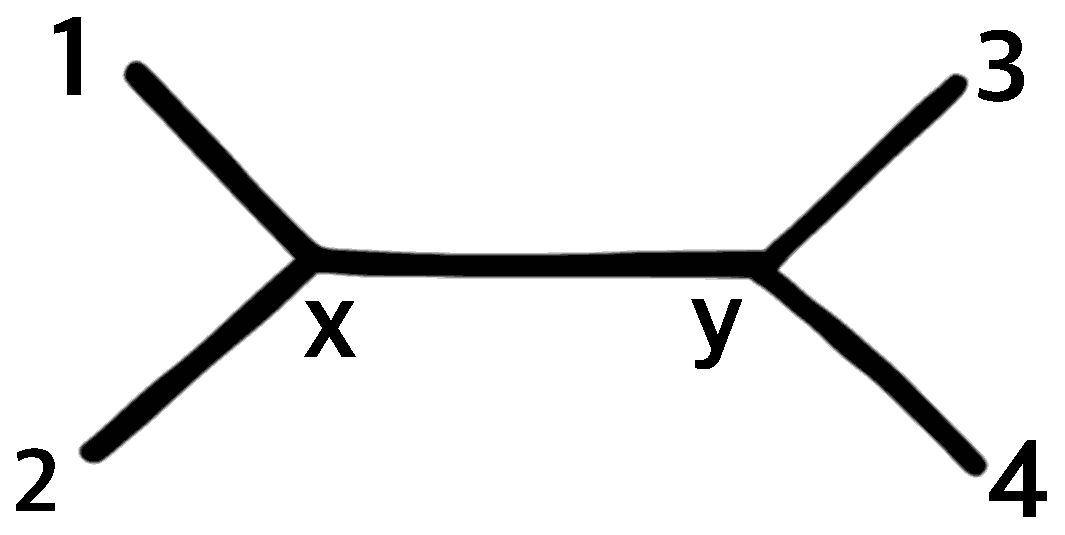
\includegraphics[width=4cm,height=2cm]{quartet12x34y.eps}
\end{figure}

\item Compute the matrices of counts between all pairs of the three
  sequences: $x_{12}, x_{13}, x_{23}$, and simulate the branch length between
  each pair with Tamura-Nei (TN) model, and $\eta=0.5$ (see JCvsTN.pdf for
  details on choosing TN and $\eta$): $d_{12},d_{13},d_{23}$
\item Compute the distances between $seq_1,seq_2$ and its parent $x$:
\begin{align*}
  d_{1x} &= \frac{(d_{12}+d_{13}-d_{23})}{2} \\
  d_{2x} &= \frac{(d_{12}+d_{23}-d_{13})}{2}
\end{align*}
\item Convert $seq_1,seq_2,seq_3,seq_4$ to matrices like
\begin{center}
\texttt{Cat ATGTTCAT...}\\[0.5cm]
$S_{cat}=$
\begin{tabular}{cccccccc}
A & 1 & 0 & 0 & 0 & 0 & 0 & 1 ...\\
C & 0 & 0 & 0 & 0 & 0 & 1 & 0 ...\\
G & 0 & 0 & 1 & 0 & 0 & 0 & 0 ...\\
T & 0 & 1 & 0 & 1 & 1 & 0 & 0 ...
\end{tabular}
\end{center}
\item Estimate the sequence distribution at $x$ from the sequences
  $seq_1,seq_2$. The formula for the likelihood at site $j$ for node
  $x$, parent of $1,2$ is:
\begin{align*}
L^x_j(s) &= \left[ \sum_{i \in \{A,C,G,T\}} P_{si}(d_{1x}) L^1_j(i)
\right] * \left[ \sum_{i \in \{A,C,G,T\}} P_{si}(d_{2x}) L^2_j(i)
\right] \\
s &\in \{A,C,G,T\}
\end{align*}
where
\begin{align*}
L^k_j(i) &= S_k[i,j], k=1,2 \\
P(t) &= \exp(\hat{Q}t)
\end{align*}

So that the sequence matrix for $x$ is given by $S_x$:
\begin{align*}
S_x[i,j] = \frac{\pi_i L^x_j(i)}{\sum_{i=1}^4 \pi_i L^x_j(i)}
\end{align*}
% \begin{center}
% $S_x=$
% \begin{tabular}{cccccccc}
% A & $L^x_1(A)$ & $L^x_2(A)$...\\
% C & $L^x_1(C)$ & $L^x_2(C)$...\\
% G & $L^x_1(G)$ & $L^x_2(G)$... \\
% T & $L^x_1(T)$ & $L^x_2(T)$...
% \end{tabular}
% \end{center}

\item Compute the count matrix between $seq_3,seq_4$: $x_{34}$ and
  simulate the branch length $d_{34}$ with TN model and
  $\eta=0.5$
\item Compute the equivalent to the count matrix between $x$ and
  $seq_3,seq_4$:
\begin{align*}
x_{x3}=\sum_{j=1}^{nsites} S_3[,j]*S_x[,j]^T
\end{align*}
\item Simulate branch lengths $d_{3x}, d_{4x}$ with TN model
  and $\eta=0.5$
\item Compute the distances between $seq_3,seq_4$ and its parent $y$,
  and between $x,y$:
\begin{align*}
  d_{3y} &= \frac{(d_{34}+d_{3x}-d_{4x})}{2} \\
  d_{4y} &= \frac{(d_{34}+d_{4x}-d_{3x})}{2} \\
  d_{xy} &= \frac{(d_{3x}+d_{4x}-d_{34})}{2}
\end{align*}

\item Compute the density of the branch lengths given the topology,
  denoted as $f_{TN}(d|T)$ for
  $d=(d_{1x},d_{2x},d_{xy},d_{3y},d_{4y})$.  We simulate the branch
  lengths: $d_{12},d_{13},d_{23},d_{3x},d_{4x},d_{34}$ with the TN
  model as gamma random variables. If we assume these 6 branch lengths
  are independent \falta{(are they?)}, the joint density is given by
  \begin{align*}
    f(d_{12},d_{13},d_{23},d_{3x},d_{4x},d_{34}) &= \prod_{i}
    \frac{\beta_i^{\alpha_i}}{\Gamma(\alpha_i)} d_i^{\alpha_i-1} \exp{(-\beta_id_i)}
  \end{align*}

  We then transform those branch lengths into the desired parameters
  (keeping the variable $d_{13}$ for the transformation to be
  bijective):
  \begin{align*}
    d_{1x} &= \frac{(d_{12}+d_{13}-d_{23})}{2} \\
    d_{2x} &= \frac{(d_{12}+d_{23}-d_{13})}{2} \\
    d_{13} &= d_{13} \\
    d_{3y} &= \frac{(d_{34}+d_{3x}-d_{4x})}{2} \\
    d_{4y} &= \frac{(d_{34}+d_{4x}-d_{3x})}{2} \\
    d_{xy} &= \frac{(d_{3x}+d_{4x}-d_{34})}{2}
  \end{align*}
  
  The determinant of the Jacobian in absolute value is $4$. Thus, the
  joint density for the transformed variables is
  \begin{align*}
    f(d_{1x},d_{2x},d_{3y},d_{4y},d_{xy},d_{13}) &=
    \left[ \prod_i \frac{\beta_i^{\alpha_i}}{\Gamma(\alpha_i)} \right] (d_{1x}+d_{2x})^{\alpha_{12}-1}
    \exp{(-\beta_{12}(d_{1x}+d_{2x}))} \\
    &* d_{13}^{\alpha_{13}-1}\exp{(-\beta_{13}d_{13})} \\
    &* (d_{13}-d_{1x}+d_{2x})^{\alpha_{23}-1}\exp{(-\beta_{23}(d_{13}-d_{1x}+d_{2x}))}\\
    &* (d_{3y}+d_{xy})^{\alpha_{3x}-1}\exp{(-\beta_{3x}(d_{3y}+d_{xy}))} \\
    &*(d_{4y}+d_{xy})^{\alpha_{4x}-1}\exp{(-\beta_{4x}(d_{4y}+d_{xy}))} \\
    &* (d_{3y}+d_{4y})^{\alpha_{34}-1}\exp{(-\beta_{34}(d_{3y}+d_{4y}))} *4
  \end{align*}

  We want to integrate out $d_{13}$,
  \begin{align*}
    f_{TN}(d_{1x},d_{2x},d_{3y},d_{4y},d_{xy}) &= \int_0^\infty
    f(d_{1x},d_{2x},d_{3y},d_{4y},d_{xy},d_{13}) d d_{13} \\
    &=\left[ \prod_i \frac{\beta_i^{\alpha_i}}{\Gamma(\alpha_i)} \right] (d_{1x}+d_{2x})^{\alpha_{12}-1}
    \exp{(-\beta_{12}(d_{1x}+d_{2x}))} \\
    &* 4\exp{(-\beta_{23}(-d_{1x}+d_{2x}))}\\
    &* (d_{3y}+d_{xy})^{\alpha_{3x}-1}\exp{(-\beta_{3x}(d_{3y}+d_{xy}))} \\
    &*(d_{4y}+d_{xy})^{\alpha_{4x}-1}\exp{(-\beta_{4x}(d_{4y}+d_{xy}))} \\
    &*(d_{3y}+d_{4y})^{\alpha_{34}-1}\exp{(-\beta_{34}(d_{3y}+d_{4y}))} \\
    &* \int_0^\infty
    d_{13}^{\alpha_{13}-1}(d_{13}-d_{1x}+d_{2x})^{\alpha_{23}-1}\exp{(-(\beta_{13}+\beta_{23})d_{13})}
    d d_{13}
  \end{align*}
  \falta{are we keeping the constants? if not, we only need to check
    that the integral is finite (which mathematica could not do,
    unless certain conditions)}

    % Bret email: One issue is that we don't really have a
    % bijection.... For the 4-taxon tree, we generate 3 gamma random
    % variables and then 3 more; 6 rvs go to 5 branch lengths. As the
    % tree gets bigger, this difference gets bigger. We discard the
    % distance from the cherry parent to the other node. At one point I
    % considered saving it, but this made the rest of the algorithm
    % messy if we had to keep track of this distance. So, if we add each
    % of these as sort of an auxiliary rv, then we can get the
    % bijection. For the density of the actual branch lengths, we
    % integrate out the auxiliary rvs and hopefully get the same
    % answer.
\end{enumerate}

\paragraph{Importance weight.} Let $p(T)$ denote the prior
distribution of tree $T$ \falta{(for topology only, or with bl?)}, and
let $L(T,d)$ denote the likelihood of $T$ under the GTR model.
\begin{align*}
L(T,d) &= \prod_k L_k(T,d) \\
L_k(T,d) & = \sum_{i=1}^4 \sum_{j=1}^4 \pi_i P_{ij}(d_{xy}) P_{i1}(d_{1x}) P_{i2}(d_{2x}) P_{j3}(d_{3y}) P_{j4}(d_{4y})
\end{align*}
\falta{(likelihood correct?)}

Then, the importance weight is
\begin{align*}
w(T) &= \frac{p(T)L(T,d)}{g(T)} \\
g(T) &= p_{ccd}(T) f_{TN}(d | T)
\end{align*}


\begin{algorithm}
\caption{Importance sampling}
\label{someAlg}

\textbf{Input:} PHYLIP or NEXUS file with DNA sequences for 4 taxa;
likelihood model (e.g. GTR) and prior

- Compute the conditional clade probabilities by bootstrapping and NJ: $p_{ccd}$

- \For{$i=1$ \KwTo $N$}{

- Sample a topology $T \sim p_{ccd}$

- Sample branch lengths from TN model $d|T \sim f_{TN}(d|T)$

- Compute importance weight $w(T)$ with likelihood and prior

}

- Normalize importance weights

% - \uIf{something}{

% - Do this

% }

% - \Else{

% - Do that

% }

\end{algorithm}


\end{document}